% !TeX spellcheck = en_GB
~
\pagebreak

\section{Automatic index updating} \label{automatic_indexing_chapter}

\begin{figure}[ht]
	\centering
	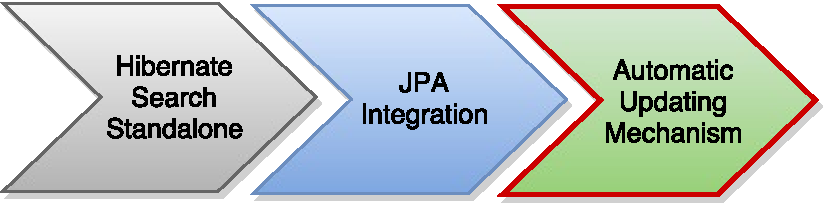
\includegraphics[scale=0.75]{images/timeline_genericjpa_third.pdf}
	\label{project_timeline_third}
\end{figure}
\noindent
As already stated in \ref{automatic_indexing_problematic_intro}, the automatic index updating feature is a required for a reasonable Hibernate Search GenericJPA. As this is arguably the most complicated feature for GenericJPA, we will go into detail about how we are achieving it next. We will start by giving a description of the different implementations available and then decide which ones to use. After that we will also give a short comparison of the pros and cons of the chosen approaches.

\pagebreak

\subsection{Description of different implementations} \label{description_of_different_implementations}

There are several approaches to building an automatic index updating feature. While they are all different in the specifics, they can generally be separated into two categories: \textbf{synchronous} and \textbf{asynchronous}. Synchronous in this context means that the index is updated as soon as the newly changed data is persisted in the database without any real delay while in an asynchronous updating mechanism an arbitrary amount of time passes before the index is updated. While synchronous approaches are needed in some rare cases, fulltext search generally doesn't require a 100\% up-to-date index at every point in time  as a search index generally is not the source of truth in an application (only the database contains the "truth").
\\\\
We will now work out a solution for both sync and async, while the async version will serve as a backup whenever the synchronized mechanism is not applicable.

\pagebreak

\subsubsection{Synchronous approach}

For the synchronous approach we have two candidates: A system based on JPA callback events and another one that uses the native APIs of JPA providers. We start with the JPA callbacks and then go onto the native APIs.

\paragraph{JPA events}

As we are trying to work with as little vendor specific APIs, JPA's callback events looks like a suitable candidate for listening to changes in entities.
\\\\
To listen for the JPA events we have two options: annotate the entities with callback methods or create a separate listener class. We will only take a look at the listener class since we don't want to have unnecessary methods in a possible user's entities. This class doesn't have to implement an interface, but has to have methods annotated with special annotations. The relevant ones are @PostPersist, @PostUpdate, @PostDelete (there are "pre-versions" available as well, but we focus on the post methods as they are more useful). What each specific annotation stands for is quite self-explanatory.
\\\\
Such a class generally looks like this:
\\
\lstset{language=java}
\lstset{moredelim=[is][\bfseries]{[*}{*]}}
\begin{lstlisting}[frame=htrbl, caption={Example JPA entity listener}, label={lst:jpa_entity_listener.java}]
public class EntityListener {

	@PostPersist
	public void persist(Object entity) {
		//handle the event
	}
	
	@PostUpdate
	public void update(Object entity) {
		//handle the event
	}
	
	@PostDelete
	public void delete(Object entity) {
		//handle the event
	}

}
\end{lstlisting}

\pagebreak

\noindent
This EntityListener is then applied with an annotation on the entity:
\\
\lstset{language=java}
\lstset{moredelim=[is][\bfseries]{[*}{*]}}
\begin{lstlisting}[frame=htrbl, caption={Using a JPA entity listener}, label={lst:using_jpa_entitylisteners.java}]
[*@EntityListeners( { EntityListener.class } )*]
public class Book {

	//...

}
\end{lstlisting}
\noindent
As the JPA provider creates the EnityListeners automatically, we have no access to them without injecting a reference to them in a static way. While this might cause some Classloader problems, it should be fine in most cases.
\\
\lstset{language=java}
\lstset{moredelim=[is][\bfseries]{[*}{*]}}
\begin{lstlisting}[frame=htrbl, caption={Injecting the EntityListener}, label={lst:jpa_entity_listener.java}]
public class EntityListener {

	public EntityListener() {
		// inject it somewhere
		// so we can access it in a static way
		EntityListenerRegistry.inject(this);
	}

	//...

}
\end{lstlisting}

\pagebreak

\noindent
Even though these listeners seem to be the perfect fit as they would enable us to fully integrate only with JPA interfaces, they have two big issues as we find out after investigating further.
\\\\
Firstly, not all JPA providers seem to handle these events similarly: For example Hibernate ORM doesn't propagate events from collection tables to the owning entity, while EclipseLink does (EclipseLink's behaviour would be needed from all providers).

Secondly, we can see that the events are triggered on flush instead of commit. This is an issue if the changed data is not actually commited.
\\

\lstset{language=java}
\lstset{moredelim=[is][\bfseries]{[*}{*]}}
\begin{lstlisting}[frame=htrbl, caption={Event triggering on flush}, label={lst:flush_event.java}]
EntityManager em = ...;

em.getTransaction().begin();

Book book = em.find( Book.class "someIsbn" );
book.setTitle( "someNewTitle" );

// flushes, so we retrieve the Book with the changes from above
// => event is triggered
List<Book> allBooks = 
	em.createQuery( "SELECT b FROM Book b" ).getResultList();

// we have no way to get this event to revert the wrong index change
em.getTransaction().rollback();
\end{lstlisting}

\noindent
While it \textbf{might} be possible to somehow fix the flush issue, the bad support from JPA providers like Hibernate ORM renders this approach unusable until the JPA providers work the same way to some reasonable extent.

\pagebreak

\paragraph{Native integration with JPA providers}

Almost every JPA provider has its own internal event system that is useful for cache invalidation and other tasks. These combined with hooks into the transaction management allow us to build a proper index updating system that works with transactions in mind (big improvement compared to the flush() issues of plain JPA)
\\\\
They generally have callbacks similar to these of the JPA events (no knowledge about database specifics is needed, Java types are used), but also provide additional information about the database session that caused the changes.
\\\\
By definition, these kind of integrations are not portable between JPA providers and require us to write different systems for all the JPA providers. But as the landscape for popular JPA providers probably only consists of Hibernate ORM, EclipseLink and OpenJPA, we can implement listeners for these and the others will have to rely on the async backup approach (as of the time of writing this, we have only implemented integrations for Hibernate ORM and EclipseLink).
\\\\
As this seems to be the only reasonable solution for a synchronous update system, we are using it for Hibernate Search GenericJPA even though it is no real native solution because of the JPA implementation dependent code.
\\\\
\textit{Note: we don't describe how these event systems are built in particular as they differ a lot in their APIs, but generally these are straightforward to use and describing the implementations would be unspectacular.}

\pagebreak

\subsubsection{Asynchronous approach}\label{async_approach}
In contrary to the synchronous approach where we described two different versions, for the asynchronous version we only have one feasible solution available: A trigger based system.
\\\\
Paul DuBois writes in MySQL - Developer's Library:
\begin{quote}
	A Trigger is a stored program that is associated with a particular table and is defined to activate for INSERT, DELETE or UPDATE statements for that table. A trigger can be set to activate either before or after each row processed by the statement. The trigger definition includes a statement that executes when the trigger activates.
	\\\\
	~[...]~
	\\\\
	A trigger can examine the current contents of a row before it is deleted or updated. This capability can be exploited to perform logging of changes [...].
	\footnote{MySQL - Developer's Library, see~\cite{mysql_developers_lib}}
\end{quote}
\noindent
While the quote above is meant to be for MySQL databases, many other RDBMS support at least triggers on the three crucial events for event-listening: INSERT (CREATE), UPDATE, DELETE, just like MySQL \footnote{CREATE TRIGGER in PostgreSQL, see~\cite{postgres_triggers}} \footnote{Triggers in HSQLDB, see~\cite{hsqldb_triggers}} \footnote{Triggers in Firebird, see~\cite{firebird_triggers}}.
\\\\
In order to have triggers being useful for updating our Hibernate Search index, we have to get info about the events from the database back into our Java application. Since we cannot necessarily call Java code from our database (with the exception of some enterprise and in-memory databases), we have to write data about changes into auxiliary tables and then poll these regularly.
\\\\
One benefit of this approach is that by using polling from the tables and the - by definition transactional - triggers, we don't have to hook into transactions or deal with data that has not been committed, yet, in general. If we do things right, we can even improve indexing performance by this: We can query for the latest event for each entity only, so we don't use up an unnecessary amount of CPU-time, but still keep the index up-to-date.

\pagebreak

\paragraph{Trigger architecture}

Triggers are generally created on tables. Since we want to use them for event-listening, we have to cover every table of the domain model that contains data indexed/stored in the index. This also includes all of the mapping tables between entities and all other secondary tables.
\\\\
The following figure \ref{triggers_schema} shows the trigger architecture needed for our Author and Book example. Also note that we are using Triggers that execute before changes are persisted.
\\
\begin{figure}[ht]
	\centering
	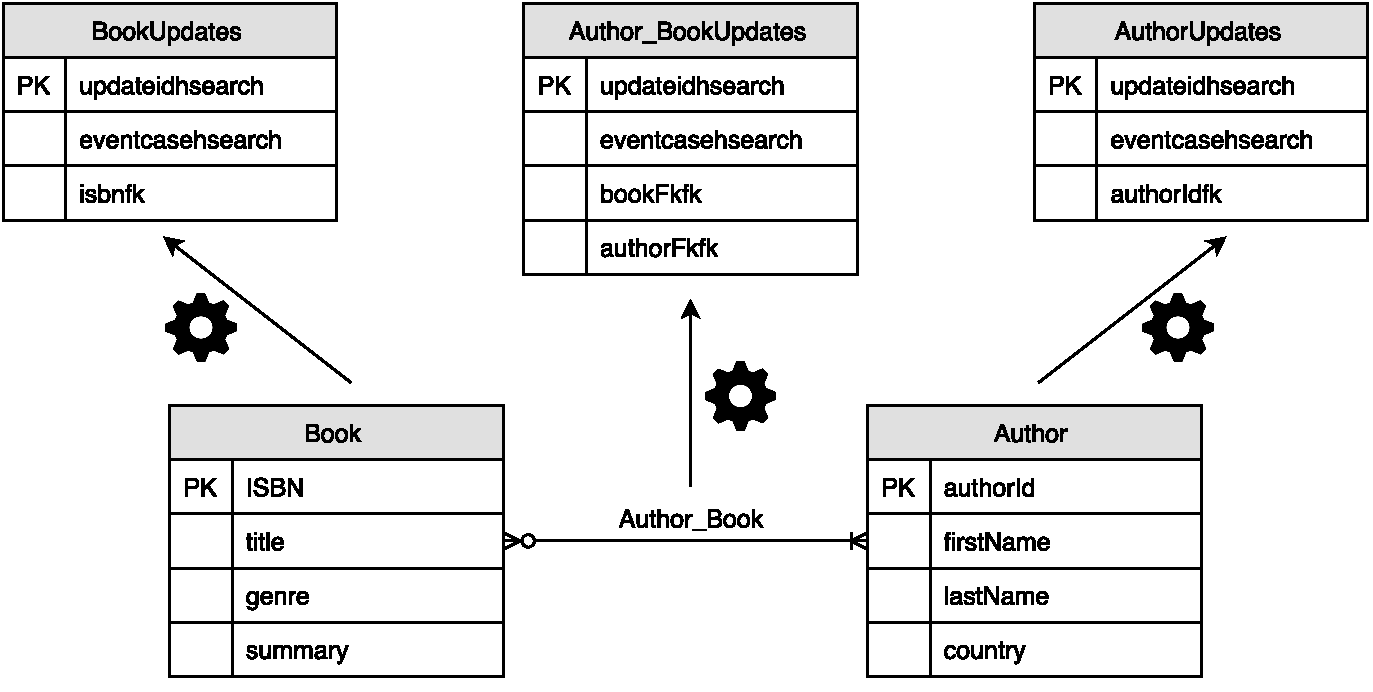
\includegraphics[scale=0.6]{images/Triggers_Schema.pdf}
	\caption{Triggers for the example project}
	\label{triggers_schema}
\end{figure}
\\
\noindent
All three tables Author, Book and Author\_Book have three triggers registered on them (one for each event type). These triggers then fill up the update tables AuthorUpdates, BookUpdates and Author\_BookUpdates (these names are just for demonstrative purposes) with info about occurring events. We can see that these update tables host at least three things:

\begin{enumerate}
	\item \textbf{updateid primary key:} Update events have to be sortable by the order they occured. All Update tables share the same sequence of primary keys so that no key appears twice in all of these tables.
	\item \textbf{eventcase column:} This column contains a identifier for the cases INSERT, DELETE or UPDATE.
	\item \textbf{pseudo foreign key(s):} The relevant primary keys of the entities involved in the tables have to be stored in the Update tables as well. Note that they are not marked as real foreign keys as a DELETE event wouldn't work then (we can't have a reference to a non existent entity).
\end{enumerate}

\pagebreak

\paragraph{Table creation} \label{creating_the_tables}

Since the creation of these tables requires a lot of work to be done, we have to automate it as good as possible. We do this by requiring additional \textbf{@UpdateInfo} annotations on the entities to map the required information for the update tables and then generating them out of it.
\\\\
These annotations contain at least the original table's name (UpdateInfo\#tableName) and the names \& types (IdColumn\#column \& IdColumn\#columnType) of the entity key columns. The name of the update table and the columns in it are then generally derived automatically from that. 
\\\\
A similar behaviour could be achieved by using the JPA mapping annotations to read the original schema and then deduce the needed update schema from that. We don't use this approach nonetheless, because the task of parsing these annotations correctly would be prone to errors due to the amount of different annotations (@Basic, @Column, @IdClass, @EmbeddedCollection, @OneToOne, @ManyToOne, @OneToMany, @ManyToMany, ...). While working out a correct solution for all the different cases would be possible, it would be quite time-consuming and wouldn't have fit in the time schedule of this thesis. However, this does not mean that we won't try to build it in the future.

\pagebreak
\noindent
The following listings show the @UpdateInfo annotation in use:
\\
\lstset{language=java}
\lstset{moredelim=[is][\bfseries]{[*}{*]}}
\begin{lstlisting}[frame=htrbl, caption={Book.java with Hibernate Search annotations}, label={lst:book.java_3}]
@Entity
@InIndex
@Table(name = "Book")
@Indexed
[*@UpdateInfo(
	tableName = "Book", 
	idInfos = @IdInfo(
		columns = @IdColumn(
			column = "isbn", 
			columnType = ColumnType.STRING
		)
	)
)*]
public class Book {

	// ... unchanged. 
	
	// mapping table events handled on Author side
	
	// getters & setters ...
}
\end{lstlisting}

\pagebreak

\lstset{language=java}
\lstset{moredelim=[is][\bfseries]{[*}{*]}}
\begin{lstlisting}[frame=htrbl, caption={Author.java with Hibernate Search annotations}, label={lst:author.java_3}]
@Entity
@InIndex
@Table(name = "Author")
[*@UpdateInfo(
	tableName = "Author", 
	idInfos = @IdInfo(
		columns = @IdColumn(
			column = "authorId", 
			columnType = ColumnType.LONG
		)
	)
)*]
public class Author {
	
	// ... unchanged.
	
	[*@UpdateInfo(tableName = "Author_Book", 
		idInfos = {
		@IdInfo(entity = Author.class, 
			columns = @IdColumn(
				column = "authorFk",
				columnType = ColumnType.LONG
			)
		),
		@IdInfo(entity = Book.class,
			columns = @IdColumn(
				column = "bookFk",
				columnType = ColumnType.STRING
			)
		)
	})*]
	private Set<Book> books;
	
	//getters & setters ...
}
\end{lstlisting}
\noindent
\textit{Note: The update tables are NO JPA entities, so we have to work with native SQL in the backend}
\\\\
\noindent
However, if the developer needs different names in the update tables (e.g. if there already exists a table with the same name), it is possible to manually set these properties. They can be found on the same level as the corresponding info for the original table is set.

\pagebreak

\noindent
Options for multivalued keys and custom column types are also available as by default only singular valued keys of the column types corresponding to Java's Integer, Long and String are supported. While we don't go into detail how these expert features are used, information about how to use them can be found in the Javadoc of the annotations.
\\\\
Since database triggers and tables are not created the same on every RDBMS, we have to build an abstraction to get the necessary SQL code. This is done with the \textbf{TriggerSQLStringSource} interface. Its implementations return the specific SQL strings working on the corresponding RDBMS. As of this writing we have implementations for MySQL, PostgreSQL and HSQDLB. See table \ref{table:config_properties_jpasearchfactorycontroller} for information about how to set the correct one for each database.
\\\\
Whether and how the triggers and tables are generated at all can also be set, but with a configuration property on the SearchFactoryController as described in table  \ref{table:config_properties_jpasearchfactorycontroller}. If disabled, the user still has to provide the information about the update tables that should be used for updating with the annotations as described above.

\pagebreak

\paragraph{Event retrieval}
Now that we know how the events are stored in the update tables, we will now describe an efficient way to query the database for these entries.
\\\\
We only need the latest event for each entity (or combination of entities for mapping tables). The following SQL query shown in listing \ref{lst:querying_updates.sql} is doing this for the table author\_bookupdates with standard SQL that should be working on every RDBMS:
\\
\lstset{language=sql}
\lstset{moredelim=[is][\bfseries]{[*}{*]}}
\begin{lstlisting}[frame=htrbl, caption={Querying for updates (Author\_Book)},
label={lst:querying_updates.sql}]
SELECT t1.updateidhsearch, t1.authorFkfk, t1.bookFkfk
FROM author_bookupdates t1
INNER JOIN
(
	/* select the most recent update */
	SELECT max(t2.updateidhsearch) updateid, 
		t2.authorFkfk, t2.bookFkfk
	FROM author_bookupdates t2
	GROUP BY t2.authorFkfk, t2.bookFkfk
) t3 on t1.updateidhsearch = t3.updateid
/* handle events that occured earlier first */
ORDER BY t1.updateidhsearch ASC;
\end{lstlisting}
\noindent
We run queries of this type for every update table with fixed delays (configurable, see table \ref{table:config_properties_jpasearchfactorycontroller}). Then, we scroll from the results
of these queries simultaneously while ordering by the updateids between the queries to make sure the events are definitely handled in the right order (see listing \ref{lst:MultiQueryAccess.java} in the appendix).
\\\\
This information is all we need to keep our index up-to-date. For the INSERT and UPDATE case we can just query the database for a new version and pass that to the engine. For the DELETE case we have to work directly on the index and have to enforce  \textbf{@IndexedEmbedded\#includeEmbeddedObjectId = true}. This is required so that we can determine the root entity in the index as its entry has to be updated additionally if the original entity is changed (An entity contained in one index can have its own index as well).

\pagebreak
\noindent
After the index is updated accordingly, we run a delete query that deletes all update events
having an updateid lower than the last processed one for each table.
\\\\
Note that we don't use a TRUNCATE statement for the query shown in the following listing \ref{lst:deleting_updates.sql} as it was only introduced with the SQL:2008 standard \footnote{Truncate statement PostgreSQL docs, see~\cite{postgres_truncate}}, which some RDBMSs don't fully support \footnote{Firebird conformance, see~\cite{firebird_conformance}}. Using TRUNCATE could therefore be a deal-breaker for some people wanting to use Hibernate Search GenericJPA. With the DELETE FROM query we make sure the clean-up statement is supported by as many RDBMSs as possible (older versions included).
\\
\lstset{language=sql}
\lstset{moredelim=[is][\bfseries]{[*}{*]}}
\begin{lstlisting}[frame=htrbl, caption={Deleting handled updates (Author\_Book)},
label={lst:deleting_updates.sql}]
DELETE FROM author_bookupdates WHERE updateidhsearch < #last_handled_id#
\end{lstlisting}
\noindent
With the two queries described in this section we are able to keep the index up-to-date efficiently and also make sure that no event is handled twice.

\pagebreak

\subsection{Comparison of approaches}

We already discussed the differences of synchronous and asynchronous approaches in general earlier this chapter. The two chosen implementations differ in terms of extra work that has to be done to get them to work (user-friendliness for the developer) and features.

\subsubsection{Additional work}
Since the native event system gets the proper information about changes from the vendor side, it doesn't require a lot of information about the general structure of the domain model and tables in the database. The Trigger based system however does need extra information as it has to poll info about changes from the database as shown in \ref{updateconsumer_architecture}. This is the reason the user has to add this information as we have seen in \ref{creating_the_tables}.
\\
\begin{figure}[ht]
	\centering
	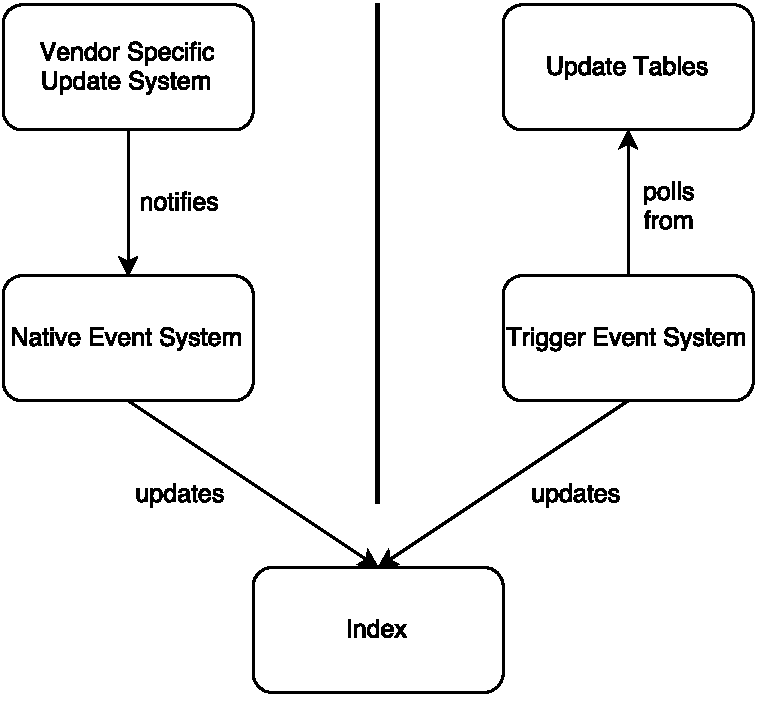
\includegraphics[scale=0.6]{images/UpdateConsumer_Architecture.pdf}
	\caption{Hibernate Search GenericJPA update mechanisms}
	\label{updateconsumer_architecture}
\end{figure}

\pagebreak

\subsubsection{Features}
The native event system has the exact same updating behaviour as Hibernate Search ORM's update mechanism because it works on the same principles of using the existing event APIs. It just works for more ORM providers.
\\\\
With this similarity come two important drawbacks:
\begin{enumerate}
	\item It (the mechanism) only works with specifically supported JPA APIs
	\item Database changes coming from anything else than JPA APIs are not recognized. This includes native SQL queries from EntityManagers. This also means that the database can only be used by the JPA application and no other scripts, small programs etc. should have write access to the database.
\end{enumerate}
\noindent
These two drawbacks are non-existent with the trigger event system as it doesn't require any specific JPA implementation (1) and works on the database level (2).

\subsubsection{Conclusion}
We can see that both event systems can be useful in different cases. This is the reason we use both in Hibernate Search GenericJPA. The following table summarizes the pros and cons once again:

\begin{table}[h] 
	\centering
	\begin{tabular}{|c|c|c|}
		\hline 
		Approach & Pros & Cons \\ 
		\hline 
		\specialcell{Native Event System} & 
		\specialcell{+ No additional work \\ needed by the developer} & 
		\specialcell{- Relies on different\\ implementation- \\ specific APIs \\ (only works with \\ specifically supported ones) \\
					- Changes from outside\\ of the JPA provider \\are not recognized \\ (e.g. native SQL access)} \\ 
		\hline
		\specialcell{Trigger Event System} & 
		\specialcell{+ Works with any JPA \\implementation \\ (even rarely used ones) \\
					+ Changes from outside\\ of the JPA provider \\ are recognized \\ (e.g. native SQL access)} & 
		\specialcell{- Additional work by \\the developer needed \\ (annotations)} \\ 
		\hline
	\end{tabular}
	\footnotesize \caption{Pros and Cons of the two update systems}
	\label{table:pros_and_cons_update_systems}
\end{table}

\pagebreak

\section{Usage of Hibernate Search GenericJPA} \label{usage_chapter}

Having described how Hibernate Search GenericJPA works and is designed we will now take a look at how it can be used in our example project (\ref{example_project}). While having already explained this part by part in each chapter, the following is everything put together and using the async updating mechanism as described in \ref{async_approach}.

\subsection{Dependencies}

The following example needs to have at least these dependencies on the classpath:

\begin{enumerate}
	\item{EclipseLink 2.5.0}
	\item{HSQLDB 2.3.3 (in memory database)}
	\item{Hibernate Search GenericJPA}
\end{enumerate}

\pagebreak

\subsection{Entities}
First, we have to update the Entity mappings in the Java classes. We add the \textbf{@Indexed, @DocumentId, @Field, @IndexedEmbedded, @ContainedIn} as known from the original Hibernate Search ORM (\ref{setting_up_example_project}). Using Hibernate Search GenericJPA then requires us also to add the @InIndex on every entity contained in the index (\ref{using_hsearch_genericjpa_index}) and because we are using the async updating mechanism here, we have to add information about how to create the update tables as well (\ref{creating_the_tables}).
\\\\
The resulting entities with the changes highlighted look like this:
\\
\lstset{language=java}
\lstset{moredelim=[is][\bfseries]{[*}{*]}}
\begin{lstlisting}[frame=htrbl, caption={Book.java complete}, label={lst:book.java_complete}]
@Entity
@Table(name = "Book")
[*@InIndex*]
[*@Indexed*]
[*@UpdateInfo(tableName = "Book",
	idInfos = @IdInfo(
		columns = @IdColumn(
			column = "isbn",
			columnType = ColumnType.STRING)))*]
public class Book {
	
	@Id
	[*@DocumentId*]
	@Column(name = "isbn")
	private String isbn;
	
	@Column(name = "title")
	[*@Field*]
	private String title;
	
	@Column(name = "genre")
	[*@Field*]
	private String genre;
	
	@Lob
	@Column(name = "summary")
	[*@Field*]
	private String summary;
	
	@ManyToMany(mappedBy = "books", cascade = {
		CascadeType.MERGE,
		CascadeType.DETACH,
		CascadeType.PERSIST,
		CascadeType.REFRESH
	})
	[*@IndexedEmbedded(includeEmbeddedObjectId = true)*]
	private Set<Author> authors;
	
	// getters & setters ...
	
}
\end{lstlisting}

\lstset{language=java}
\lstset{moredelim=[is][\bfseries]{[*}{*]}}
\begin{lstlisting}[frame=htrbl, caption={Author.java complete}, label={lst:author.java_complete}]
@Entity
@Table(name = "Author")
[*@InIndex*]
[*@UpdateInfo(tableName = "Author", 
	idInfos = @IdInfo(
		columns = @IdColumn(
			column = "authorId",
			columnType = ColumnType.LONG
	)
))*]
public class Author {
	
	@Id
	@GeneratedValue(strategy = GenerationType.AUTO)
	@Column(name = "authorId")
	[*@DocumentId*]
	private Long authorId;
	
	@Column(name = "firstName")
	[*@Field*]
	private String firstName;
	
	@Column(name = "lastName")
	[*@Field*]
	private String lastName;
	
	@Column(name = "country")
	[*@Field*]
	private String country;
	
	@ManyToMany(cascade = {
		CascadeType.MERGE,
		CascadeType.DETACH,
		CascadeType.PERSIST,
		CascadeType.REFRESH
	})
	@JoinTable(name = "Author_Book", 
		joinColumns = @JoinColumn(name = "authorFk", 
			referencedColumnName = "authorId"),
		inverseJoinColumns = @JoinColumn(name = "bookFk",
			referencedColumnName = "isbn"))
	[*@UpdateInfo(tableName = "Author_Book",
		idInfos = {
			@IdInfo(entity = Author.class,
				columns = @IdColumn(
				column = "authorFk",
				columnType = ColumnType.LONG)),
			@IdInfo(entity = Book.class,
				columns = @IdColumn(
				column = "bookFk",
				columnType = ColumnType.STRING))
	})*]
	[*@ContainedIn*]
	private Set<Book> books;
	
	// getters & setters ...
	
}
\end{lstlisting}


\pagebreak

\subsection{persistence.xml}

The persistence.xml file for our JPA based project is straightforward. As we are using an in-memory database with HSQLDB, settings for the schema creation and the user management are not important as the database is recreated at every restart.
\\

\lstset{language=xml}
\begin{lstlisting}[frame=htrbl, caption={persistence.xml complete}, label={lst:persistence.xml_complete}]
<persistence xmlns="http://java.sun.com/xml/ns/persistence"
xmlns:xsi="http://www.w3.org/2001/XMLSchema-instance"
xsi:schemaLocation="http://java.sun.com/xml/ns/persistence
	http://java.sun.com/xml/ns/persistence/persistence_2_0.xsd"
	version="2.0">

	<persistence-unit name="EclipseLink_HSQLDB"
		transaction-type="RESOURCE_LOCAL">
		<provider>
			org.eclipse.persistence.jpa.PersistenceProvider
		</provider>
		<class>*.*.Author</class>
		<class>*.*.Book</class>
		<properties>
			<property name="javax.persistence.jdbc.driver"
				value="org.hsqldb.jdbcDriver"/>
			<property name="javax.persistence.jdbc.url"
				value="jdbc:hsqldb:mem:test"/>
			<property name="javax.persistence.jdbc.user"
				value="user"/>
			<property name="javax.persistence.jdbc.password"
				value="password"/>
			<property name="eclipselink.ddl-generation"
				value="drop-and-create-tables"/>
			<property name="eclipselink.logging.level"
				value="INFO"/>
			<property name="eclipselink.ddl-
				generation.output-mode"
				value="both"/>
		</properties>
	</persistence-unit>
	
</persistence>
\end{lstlisting}

\pagebreak

\subsection{Code usage example}

In the following listing we show the whole lifecycle of a Hibernate Search GenericJPA based application. The relevant code passages are commented in the code.
\\

\lstset{language=java}
\lstset{moredelim=[is][\bfseries]{[*}{*]}}
\begin{lstlisting}[frame=htrbl, caption={Complete usage}, label={lst:complete_usage.java}]
Properties properties = new Properties();

// use the async backend
properties.setProperty(
	"hibernate.search.searchfactory.type",
	"sql"
);

// we are using HSQLDB, so use the right TriggerSource
properties.setProperty(
	"hibernate.search.trigger.source",
	"org.hibernate.search.genericjpa.db." + 
		"events.triggers.HSQLDBTriggerSQLStringSource"
);

// start up the EntityManagerFactory (entry-point to JPA)
// and create one EntityManager
EntityManagerFactory emf = Persistence
	.createEntityManagerFactory( "EclipseLink_HSQLDB" );
EntityManager em = emf.createEntityManager();

// start up Hibernate Search GenericJPA
JPASearchFactoryController searchController = 
	Setup.createSearchFactoryController( emf, properties );

// persist entities in the database
em.getTransaction().begin();
Author author = ...;
Book book = ...;
book.setAuthor( author );
em.persist( em );
em.getTransaction().commit();

// we are using an async backend, so wait a bit
// for the updating mechanism to handle the
// persist (Exception not handled here)
Thread.sleep( 10_000 );

// create a FullTextEntityManager
FullTextEntityManager fem = searchController
	.getFullTextEntityManager( em );

// query for all Books having the title "searchString"
FullTextQuery fullTextQuery = fem.createFullTextQuery(
	fem.getSearchFactory().buildQueryBuilder()
		.forEntity( Book.class )
		.get()
		.keyword()
		.onField( "title" )
		.matching( "searchString" )
		.createQuery(), 
	Book.class);

List<Book> books = (List<Book>) fullTextQuery.getResultList();

//handle the books
System.out.println( books );

// close everything 
// (FullTextEntityManager is not closed because
// the EntityManager is closed)
em.close();
searchController.close();
emf.close();
\end{lstlisting}
\noindent
Note that we didn't put the code into a main method. This is due to the fact that in a real application all this code would obviously not be put into one single method:
\\\\
The startup process of Hibernate Search GenericJPA is generally put into an extra lifecycle helper that stores a reference to the JPASearchFactoryController in a global variable upon application startup similar to what is generally done with JPA's EntityManagerFactory (at least in Java SE applications). All Search related code then acquires the reference to the JPASearchFactoryController from the global variable and uses it similar to the above code. The lifecycle helper is also responsible for closing the JPASearchFactoryController when the application is shutting down.

\pagebreak